\chapter{Results} \label{ch:resultados}

This section provides the main results of the investigation. The main functions used to obtain these results are shown in the Appendix \ref{ch:Anexo}. 
The results are divided into three sections:
\begin{enumerate}
    \item First, the results reproduced from the original paper \cite{notarmuzi2021percolation} are presented.
    \item Secondly, we will present the same analysis for the case of a Hawkes process with $n=2$.
    \item Finally, we will study the behaviour of two coupled Hawkes process, one representing an excitatory neuron and the other an inhibitory neuron.
\end{enumerate}

\section{Results for n=1}

The structure for the three sections will be the same. First, we will obtain the phase diagram for the percolation strength $P_{\infty}$ versus our control parameter, the resolution parameter 
$\Delta$, obtaining the critical point(s) $\Delta^*_{i}$. Next, the avalanche statistics for size and duration will be studied for different regions of the phase diagram.  

As previously stated, the first result is the percolation phase diagram, shown in Figure \ref{f:phase_diagram_article} 
versus the resolution parameter $\Delta$. To obtain this plot, we generated several time series, computed the percolation strength for each one, and plotted the average across realizations.

\begin{figure}[H]
    \centering
    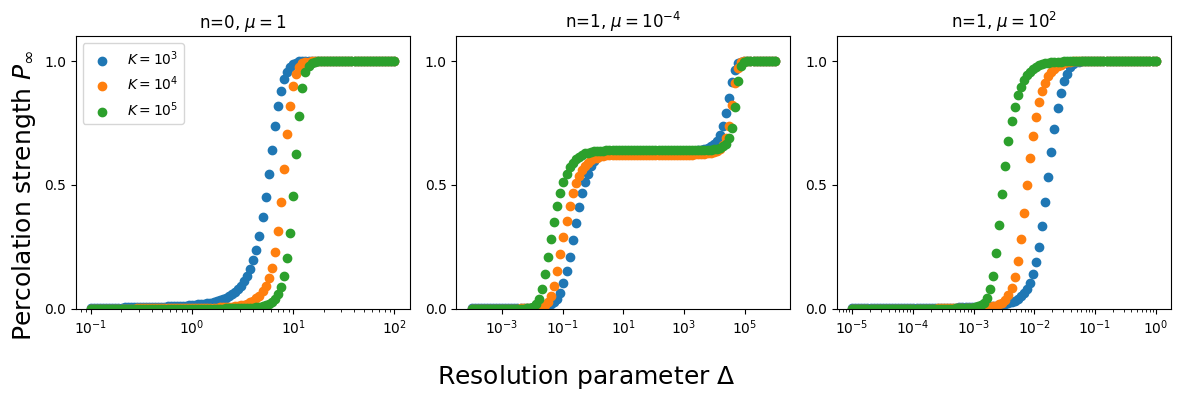
\includegraphics[width=0.95\textwidth]{phase_article_R=1000.png}
    \caption{Percolation phase diagrams for different number of events $K$ taking average values of $R=1000$ realizations. We have included the homogeneous Poisson process at the left for 
    comparison.}
    \label{f:phase_diagram_article}
\end{figure}

The first plot configuration is a homogeneous Poisson process with rate $\mu=1$ which we have overviewed in Section \ref{subsec:Poisson_processes} and has a pseudocritical threshold at 
$\Delta^*(K)=\frac{\ln(K)}{\mu}$ as we have demonstrated in Section \ref{sec:physics_cooking}. Due to the finite size of the time series, the transition is located at 
the threshold, as expected for 1D percolation \cite{stauffer2018introduction}.

Now, we will consider Hawkes processes, for the first case $\left( \mu=10^{-4} \right)$, we can observe a double transition. The first one is at $\Delta_1^*$ and the second one at 
$\Delta_2^*$. As we are going to see with the avalanche statistics, the first transition is associated with the universality class of 1D percolation, whose exponents are $\alpha=\tau=2$. 
On the other hand, the second transition is associated with the universality class of the mean-field branching process, whose exponents are $\alpha=3/2$ and $\tau=2$. This double transition 
is also compatible with what was mentioned in Figure \ref{f: Delta percolación}. We can also observe that the plateau between the two transitions is wider as the $K$ increases as expected.
For the second case $\left( \mu=10^2 \right)$, similarly to the first one, we have a single transition at $\Delta_1^*$ associated with the universality class of 1D percolation
as well; this phenomenon is also compatible with what was shown in Figure \ref{f: Delta percolación 2}.

Another interesting analysis to characterize the phases is studying the susceptibility $\chi$. Let $S_M$ be the size of the largest cluster, then the susceptibility is defined by 
Eq. \ref{eq:susceptibilidad}. 

\begin{equation}
    \begin{split}
        \chi =& \dfrac{ \langle S_M^2 \rangle - \langle S_M \rangle^2 }{\langle S_M \rangle}\\
             =& K\cdot \dfrac{\langle P_{\infty}^2 \rangle - \langle P_{\infty} \rangle^2}{\langle P_{\infty} \rangle}\\
             =& K\cdot \dfrac{\sigma^2\left( P_\infty \right)}{\langle P_{\infty} \rangle}
    \end{split}
    \label{eq:susceptibilidad}
\end{equation}

The susceptibility (normalized to the number of events) is shown in Figure \ref{f:susceptibilidad_article}. For the Poisson process, we see that the susceptibility has a peak at the
threshold $\Delta^*(K)$, then it vanishes as expected. For the Hawkes case with $\mu=10^{-4}$, we observe that $\chi$ has a peak at the critical point $\Delta_1^*$, then 
we have a critical behaviour where the susceptibility is not zero at the plateau $[\Delta_1^*,\Delta_2^*]$ and finally, it vanishes at the second critical point, $\Delta_2^*$. Finally, 
for the Hawkes case with $\mu=10^2$ and likewise the Poisson process, the susceptibility has a divergence at the critical point $\Delta_1^*$ and then it vanishes. 

\begin{figure}[H]
    \centering
    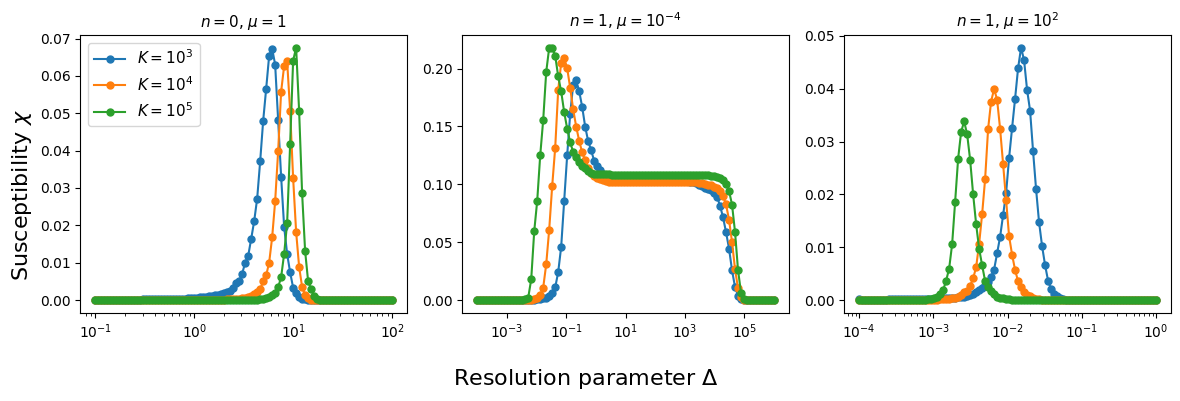
\includegraphics[width=0.95\textwidth]{susceptibilidad n=1.png}
    \caption{Susceptibility $\chi$ normalized to the number of events $K$, for different event number $K$ and taking average values for $R=1000$ realizations.}
    \label{f:susceptibilidad_article}   
\end{figure}

Once we have the phase diagram, we can study avalanche statistics, but first, we need to obtain the thresholds $\Delta_1^*$ and $\Delta_2^*$ from the phase diagram. 
The article \cite{notarmuzi2021percolation} provides the following formulas to compute these thresholds for the Hawkes process with $\mu=10^{-4}$:

\begin{align}
    \Delta_1^* &\simeq \dfrac{\ln(K)}{\langle \lambda \rangle}= \dfrac{\ln(K)}{\mu+\sqrt{2\mu K}} \label{eq:Ecuación delta1 *} \\
    \Delta_2^* &= \dfrac{\ln(K)}{\mu}\label{eq:Ecuación delta2 *}
\end{align}

and for $\mu=10^2$:

\begin{equation}
    \Delta_1^* = \dfrac{\ln(K)}{\mu}
\end{equation}

Bearing this in mind and the definitions of the size and duration of avalanches established in the previous chapter, we can study the avalanches for the different regions
of the phase diagram. We are just going to show the results for $\mu=10^{-4}$ and for $\mu=10^2$ in Figure \ref{f:avalanches_article}. The Poisson process behaviour can be found in 
\cite{stauffer2018introduction, stauffer1978critical}. 

\begin{figure}[H]
\centering
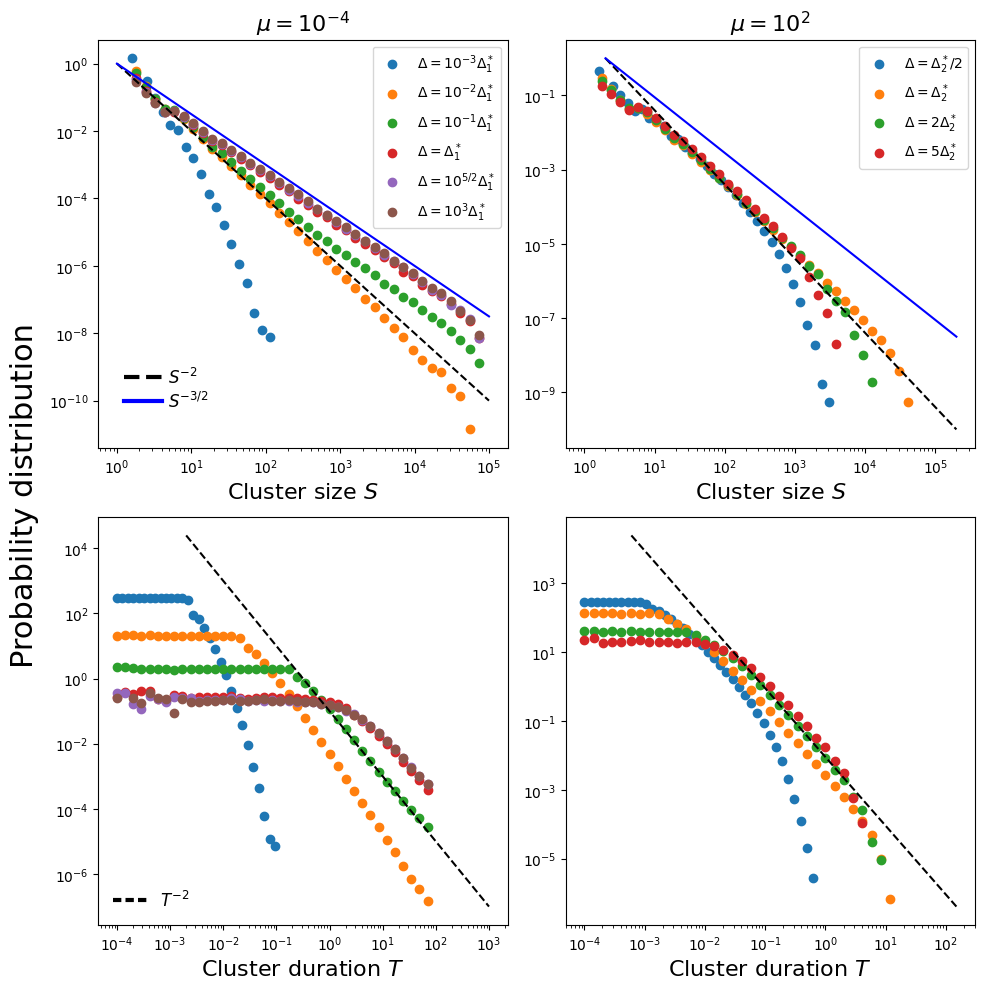
\includegraphics[width = 0.7\textwidth]{stats article.png}
\caption{Avalanche analysis for Hawkes process with $n=1$, $K=10^5$ events. The histograms have been calculated over $R=1000$ time series.}
\label{f:avalanches_article}  
\end{figure}


% \begin{wrapfigure}{l}{0.65\textwidth}
%       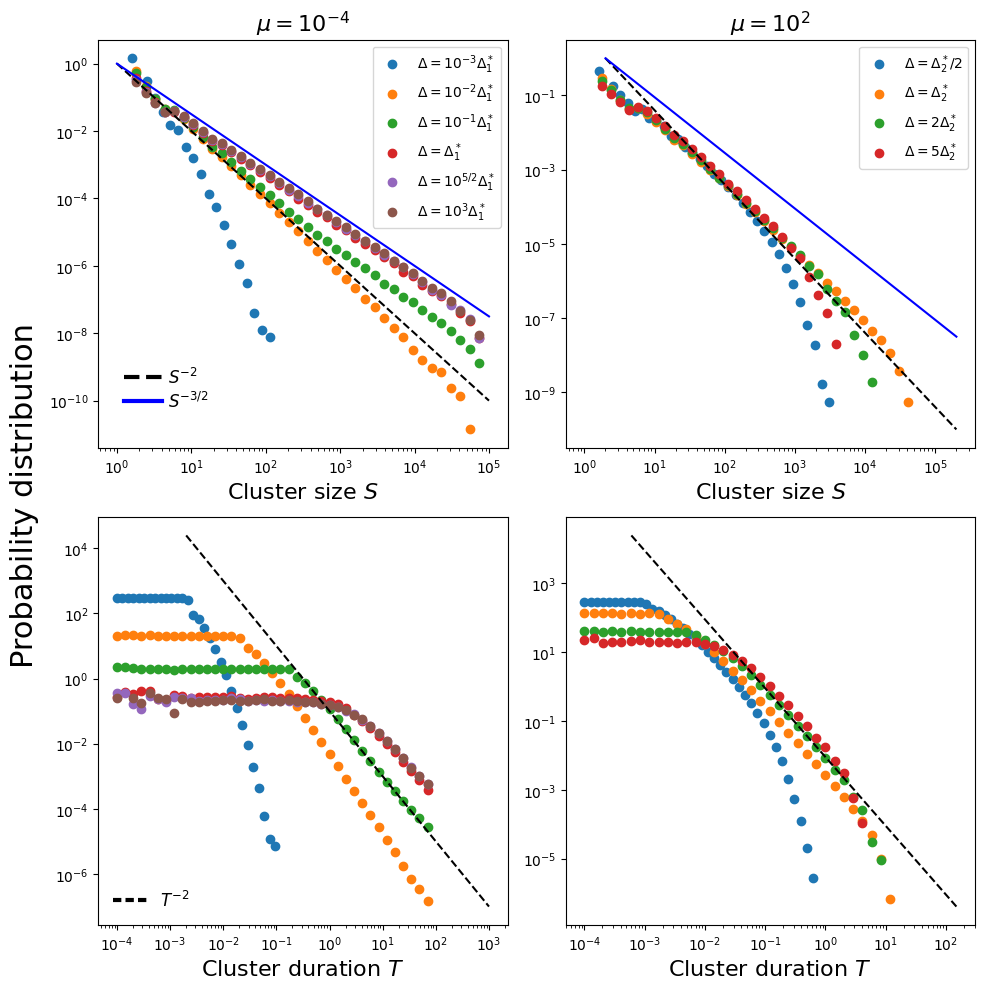
\includegraphics[width=0.6\textwidth]{stats article.png}
%     \caption{Avalanche analysis for Hawkes process with $n=1$, $K=10^5$ events. The histograms have been calculated over $R=1000$ time series.}
%     \label{f:avalanches_article}
% \end{wrapfigure}

As a consequence of the huge simulation time for time series with $K=10^8$ events, we only have studied avalanches for $K=10^5$, moreover, we have taken other criteria to obtain the 
histograms. Instead of considering $C=10^7$ clusters, we have obtained the histograms of $R=1000$ time series. This leads to a different amount of clusters for each value of $\Delta$.
Nevertheless, we have obtained equivalent and robust results.

For $\mu=10^{-4}$, the probability distribution of the cluster size and duration shows three different behaviours. For $\Delta\ll\Delta_1^*$, the behaviour is subcritical, leading to
an exponential decay for the size and duration. As we increase $\Delta$, we reach the critical point where the exponents are $\alpha=\tau=2$ compatible with the universality class
of 1D percolation. After that, we reach the plateau $[\Delta_1^*,\Delta_2^*]$ where we have a crossover to the universality class of mean-field branching process and 1D percolation. 
Finally, for $\Delta\to\Delta_2^*$, we obtain the universality class of mean-field branching process exponents $\alpha=3/2$ and $\tau=2$. 
For $\mu=10^2$, the plots show a power-law distribution for both cluster size and duration with exponents $\alpha=\tau=2$ corresponding to the universality class of 1D percolation as we have
mentioned before.

Note that we have reproduced the same behaviour, but for other values of $\Delta$, specifically, for two orders of magnitude less than in ref. \cite{notarmuzi2021percolation}. This is due 
to the fact that Eq. \ref{eq:Ecuación delta1 *} needs the assumption of large time series, which is not fulfilled in our case. 
We can illustrate this difference,
for example, in the susceptibility diagram, where the peak should be at $\Delta_1^*$, but in our case, it is at $\Delta_1^*/100$ as shown in Figure \ref{f:different delta1estrella}. 


\begin{figure}[H]
\centering
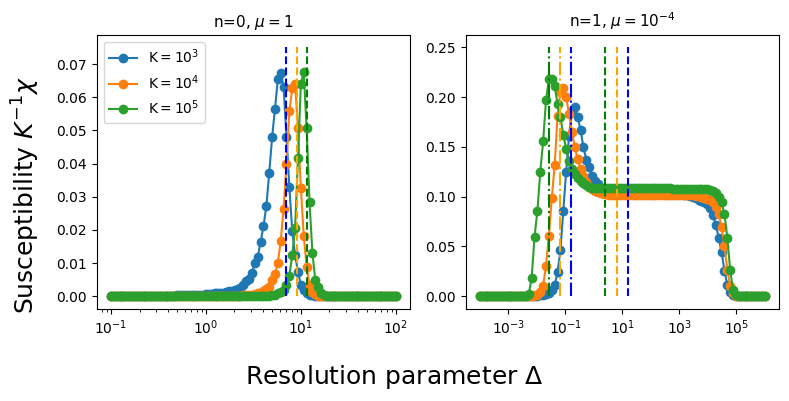
\includegraphics[width = 0.7\textwidth]{different delta1estrella.png}
\caption{On the left, the vertical dashed lines represent the critical points $\Delta^*(K)$ for the Poisson process. On the right, the vertical dashed lines represent 
the critical points $\Delta_1^*(K)$ given by Eq. \ref{eq:Ecuación delta1 *} and the dotted dashed lines the $\Delta_1^*/100$.} 
\label{f:different delta1estrella}
\end{figure}

\section{Results for n=2}

In the article, the authors have studied a process that is critical itself because the parameter $n$ is fixed to $n=1$. We have studied the case $n=2$ to see if the process is still critical. 
In Figure \ref{f:n=1 vs n=2} two event series for $n=1$ and $n=2$ are shown. 

\begin{figure}[H]
    \centering
    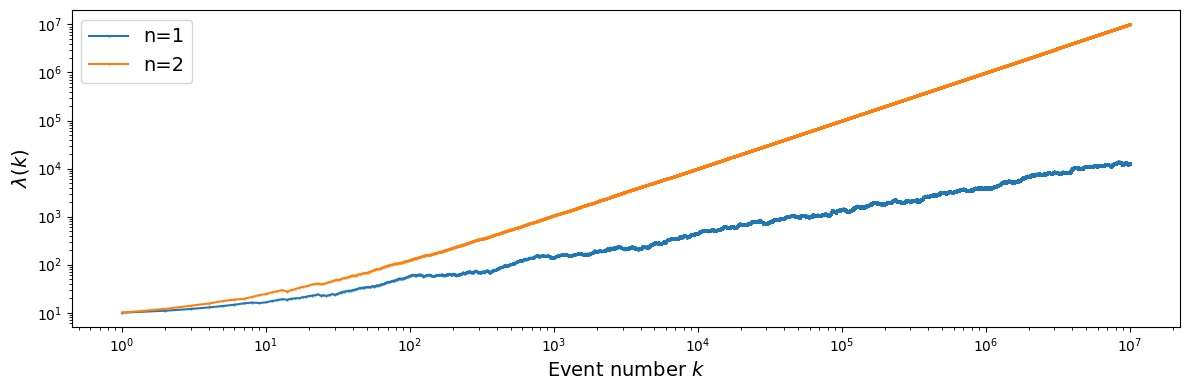
\includegraphics[width=0.7\textwidth]{n=1 vs n=2.png}
    \caption{Event series for $n=1$ and $n=2$.}
    \label{f:n=1 vs n=2}
\end{figure}

As presented in the figure above, the rate of the process for $n=2$ explodes in comparison with the rate for $n=1$. 
Similarly to the previous section, the first step is obtaining the phase diagram in order to distinguish the regimes. 

\begin{figure}[H]
    \centering
    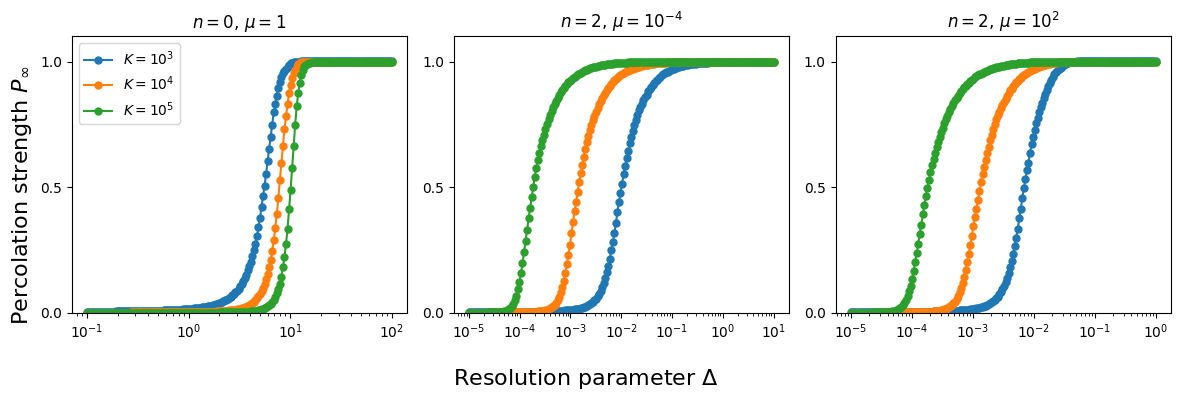
\includegraphics[width=0.95\textwidth]{phase_R=1000_n=2.png}
    \caption{Percolation phase diagrams for a Hawkes process with $n=2$ compared to the homogeneous Poisson process on the left.}
    \label{f:phase_diagram_n=2}
\end{figure}
In this case, Eqs. \ref{eq:Ecuación delta1 *},  \ref{eq:Ecuación delta2 *} are not valid because they were derived for $n=1$. 
Therefore, we will obtain this parameter graphically from the phase diagrams shown in Figure \ref{f:phase_diagram_n=2}. We will establish $\Delta^*$ at the resolution parameter where the
percolation strength $P_{\infty} = 0.5$, consequently, $\Delta^*\approx 10^{-4}$ for both cases. Like in the previous section, in Figure \ref{f:susceptibilidad_n=2} the susceptibility is shown.

\begin{figure}[H]
    \centering
    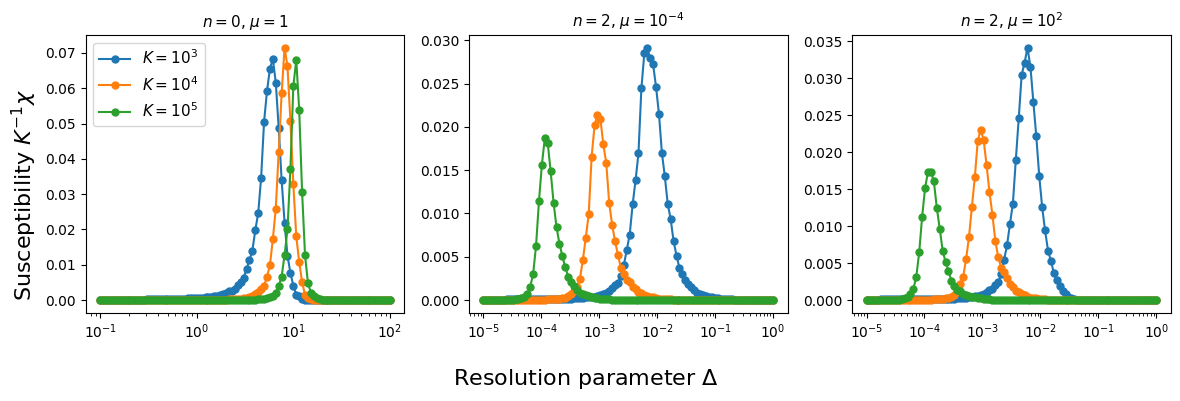
\includegraphics[width=0.95\textwidth]{susceptibilidad n=2.png}
    \caption{Susceptibility $\chi$ normalized to $K$, for different number of events and taking average values for $R=1000$ realizations.}
    \label{f:susceptibilidad_n=2}
\end{figure}


As we can recognize from both figures, now we have a single transition for $\mu=10^{-4}$ and $\mu=10^2$, in principle corresponding to 1D percolation, ergo, 
the exponents for the size and duration should be $\alpha=\tau=2$. As we did for the case with $n=1$, we have studied the avalanches for $K=10^5$ events and $R=1000$ realizations to 
obtain the histograms. The statistics of the avalanches are shown in Figure \ref{f:avalanches_n=2}.

\begin{figure}[H]
    \centering
    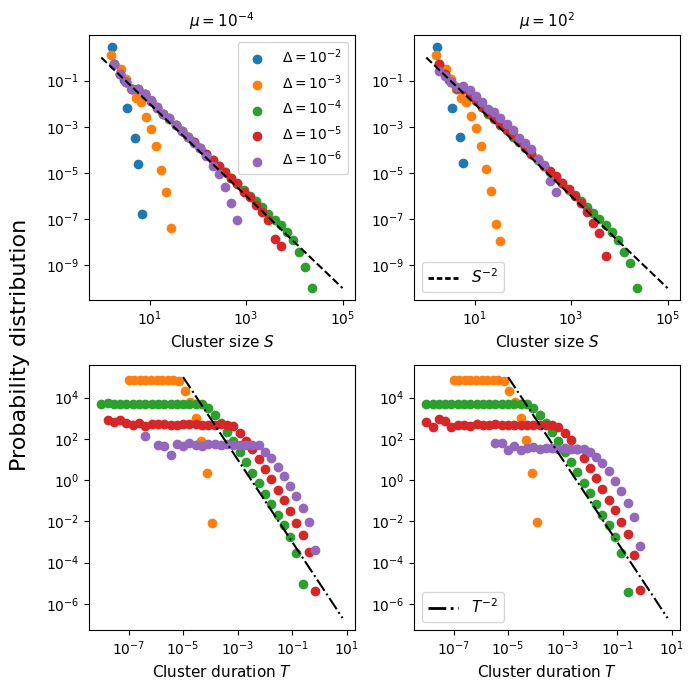
\includegraphics[width = 0.6\textwidth]{stats n=2.png}
    \caption{Avalanche statistics for a self-exciting Hawkes process with $n=2$ for $K=10^5$ events. The histograms have been calculated over $R=1000$ time series.}
    \label{f:avalanches_n=2} 
\end{figure}
    

% \begin{wrapfigure}{l}{0.6\textwidth}
%       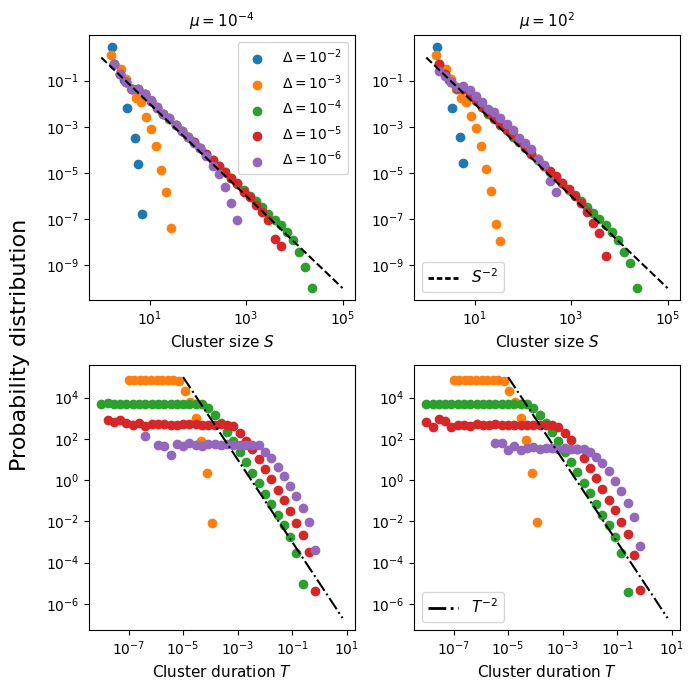
\includegraphics[width=0.58\textwidth]{stats n=2.png}
%     \caption{Avalanche statistics for a self-exciting Hawkes process with $n=2$ for $K=10^5$ events. The histograms have been calculated over $R=1000$ time series.}
%     \label{f:avalanches_n=2}
% \end{wrapfigure}

As the image shows, we have obtained the exponents $\alpha=\tau=2$ for both cases, which is compatible with the universality class of 1D percolation. This situation is analogous to the 
one shown in the case of $n=1, \mu=10$ (Figure \ref{f: Hawkes rate burst 2}) but with a more pronounced effect due to the value of $n$. Moreover, as happened with $n=1$, the cutoff 
of the power-law (caused by the finite size of $K$) for the cluster duration monotonically shifts to higher values as $\Delta$ increases.
In conclusion, we observe percolation phenomena for 
$n\neq 1$, we also observe power law distributions for the size and duration of the avalanches but not caused by criticality as we have seen in the susceptibility diagram, $\chi$ only diverges
at $\Delta^*$. 
Note that with $n=2$, we just have a single transition and its susceptibility peak. For that reason, the criticality is induced only by the order parameter $\Delta$ and not by the 
underlying dynamics, as happened when $n=1$.


\section{Results for the bivariate case with excitation and inhibition}

We will only look at two parameter 
configurations. The first one gives us a "pseudo-critical" signal, regulated by inhibition. On the other hand, the second one gives us an oscilatory and "stationary" signal. For both signals, 
the background rates will be $\mu_E=\mu_I=10^{-2}$, the other interaction parameters are shown in Table \ref{tab: Hawkes coupled parameters}.


\begin{table}[H]
    \centering
    \caption{Interaction parameters for both bivariate processes}
    \label{tab: Hawkes coupled parameters}
    \begin{tabular}{@{}ccc@{}}
    \toprule
     & \multicolumn{1}{c}{Pseudo-critical} & \multicolumn{1}{c}{Stationary} \\ \midrule
    $n_{EE}$ & 1.5 & 1.5 \\
    $n_{EI}$ & 1.5 & 1.5 \\
    $n_{IE}$ & -0.33 & -0.5 \\
    $n_{II}$ & 0 & 0 \\ \bottomrule
    \end{tabular}
\end{table}

With the value of $n_{EE}$, the signals would be supercritical, but adding the inhibition, the behaviour becomes totally different. Moreover, we will see that a 
slight change in the inhibition strength will change the signal from pseudo-critical to oscilatory. In Figures \ref{f: Hawkes coupled pseudo} and \ref{f: Hawkes coupled oscilatory}
we presente the time series and raster plots for the two different signals.

\begin{figure}[H]
    \centering
    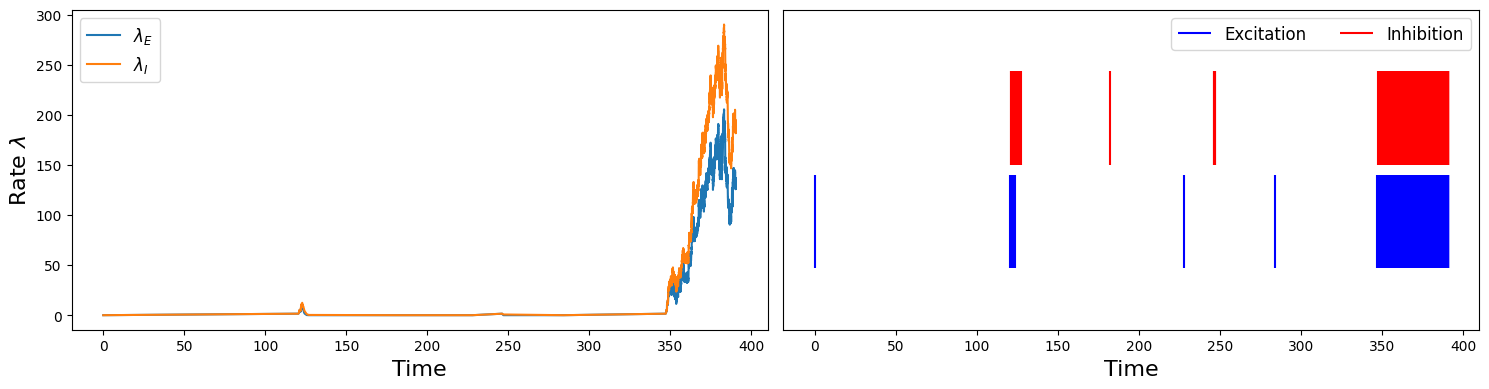
\includegraphics[width=0.95\textwidth]{raster plot bivariate critical.png}
    \caption{On the left, a temporal series of $K=10^4$ events of a bivariate Hawkes process with the interaction parameters of the pseudo-critical signal shown in Table \ref{tab: Hawkes coupled parameters},
    on the right, the raster plot of the same process for excitatory and inhibitory events.}
    \label{f: Hawkes coupled pseudo}
\end{figure}

\begin{figure}[H]
    \centering
    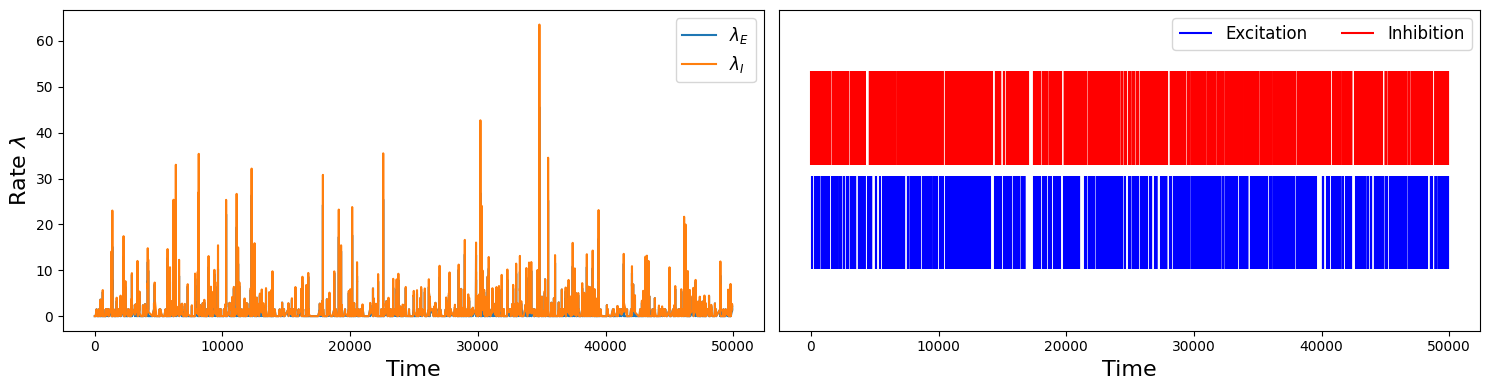
\includegraphics[width=0.95\textwidth]{raster plot bivariate stationary.png}
    \caption{On the left, a temporal series of $K=10^4$ events of a bivariate Hawkes process with the interaction parameters of the ``stationary'' signal shown in Table \ref{tab: Hawkes coupled parameters},
    on the right, the raster plot of the same process for excitatory and inhibitory events.}
    \label{f: Hawkes coupled oscilatory}
\end{figure}

As illustrated, the pseudo-critical signal has a bursty structure until a big avalanche of activity occurs; on the contrary, the ``stationary'' signal has a more regular structure.

In this case, we will only cover the case of $\mu\ll 1$. 
This is because as we have seen in Eq. \ref{eq: inter-event time coupled} $g_j$ must be positive and having $\alpha_{IE}\equiv n_{IE}<0$ leads to a negative $g_j$ sporadically. 
We have solved this issue by setting $\lambda_j(t_k)=\mu_j$ for $j=E,I$, which does not change the dynamics as it does if $\mu_j>>1$. In order to cover the case of $\mu\gg 1$ we could 
use Ogata thinning algorithm \cite{ogata1981lewis} to simulate coupled processes, but this algorithm less efficient than the one that we have used and computing the same amount of
time series would take much longer. 

Now, the main results for the case of excitatory and inhibitory processes are presented. First of all we will show the results for ``pseudo-critical'' 
signals shown in Figure \ref{f: Hawkes coupled pseudo}. Both the phase diagrams and avalanche statistics shall be calculated with the event times in general, without distinguishing
between excitatory and inhibitory events. Future work could be conducted to study the avalanches for each type of event separately. 
The phase diagram and its corresponding susceptibility 
are shown in Figures \ref{f:phase_diagram_coupled critical} and \ref{f:susceptibilidad_coupled critical} respectively. 
\begin{figure}[H]
    \centering
    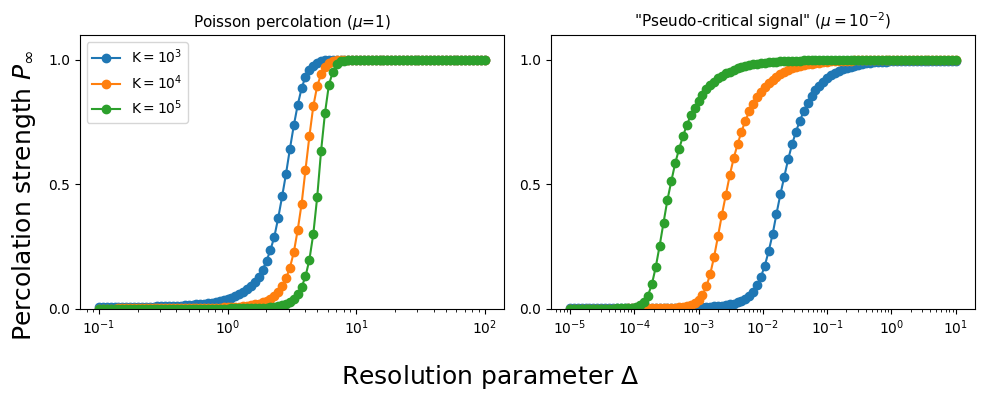
\includegraphics[width=0.8\textwidth]{phase bivariate critical 10-2.png}
    \caption{Percolation phase diagrams averaged over $R=1000$ ``pseudo-critical' signals of $K=10^5$ events. $\left( n_{EE}=n_{EI}=1.5, n_{IE}=-0.33 \right)$} 
    \label{f:phase_diagram_coupled critical}
\end{figure}

\begin{figure}[H]
    \centering
    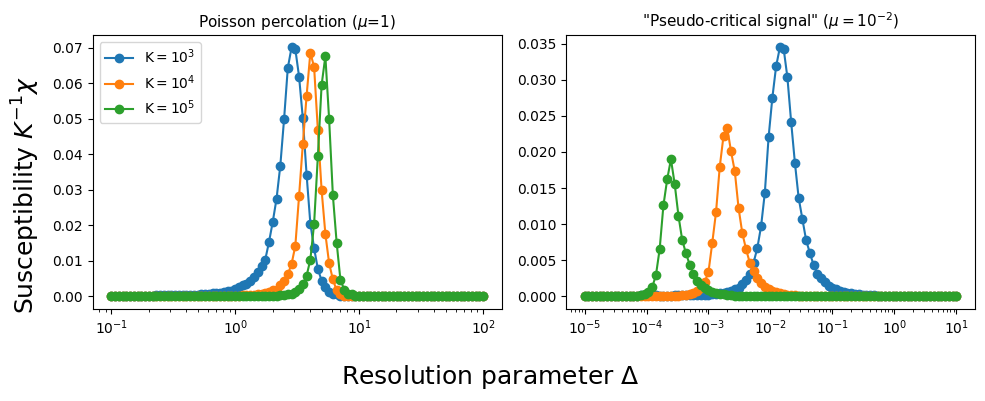
\includegraphics[width=0.8\textwidth]{susceptibilidad bivariate critical 10-2.png}
    \caption{Susceptibility $\chi$ normalized to the number of events associated with the above phase diagram.}
    \label{f:susceptibilidad_coupled critical}
\end{figure}

Both figures show a single transition around $\Delta^*\approx 2\cdot 10^{-4}$ for $10^5$ events, that so far has corresponded with the universality class of 1D percolation, but on this occasion, we have the same 
situation as in the case of $n=1$ and $\mu=10^{-4}$, as illustrated in Figure \ref{f: stats pseudocritical}.

\begin{figure}[H]
    \centering
    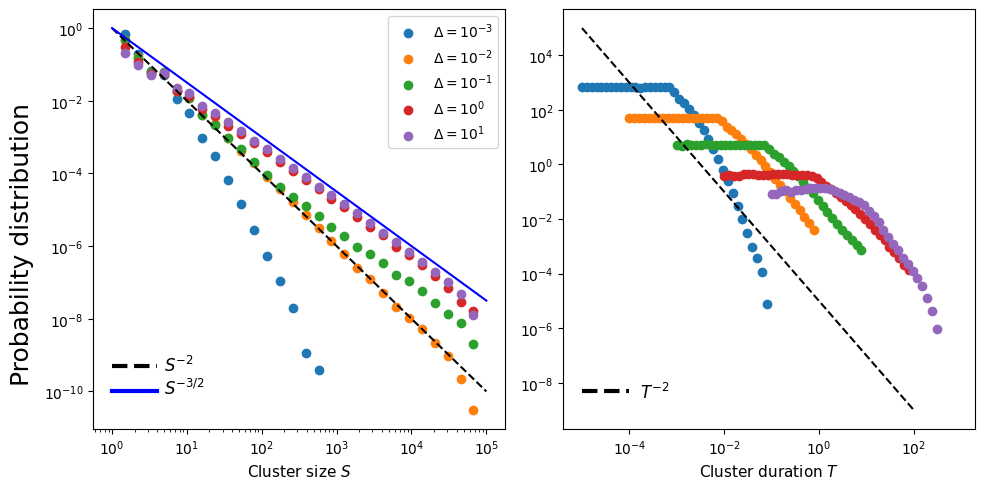
\includegraphics[width=0.8\textwidth]{stats bivariate critical 10-2.png}
    \caption{Avalanche statistics of $K=10^5$ events for ``pseudo-critical'' signals of two coupled Hawkes processes. Histograms have been calculated over $R=1000$ time series.}
    \label{f: stats pseudocritical}
\end{figure}

In this case, the exponents for the size and duration of the avalanches behave as if there was a double transition in the phase diagram, but in fact, there is not. Further analyses will be needed
to clarify this phenomenon. On the contrary, in the case of 
the ``stationary'' signal shown in Figure \ref{f: Hawkes coupled oscilatory} we do not have this anomaly. The phase diagram and susceptibility are shown in Figures 
\ref{f:phase_diagram_coupled oscilatory} and \ref{f:susceptibilidad_coupled oscilatory}, respectively.

\begin{figure}[H]
    \centering
    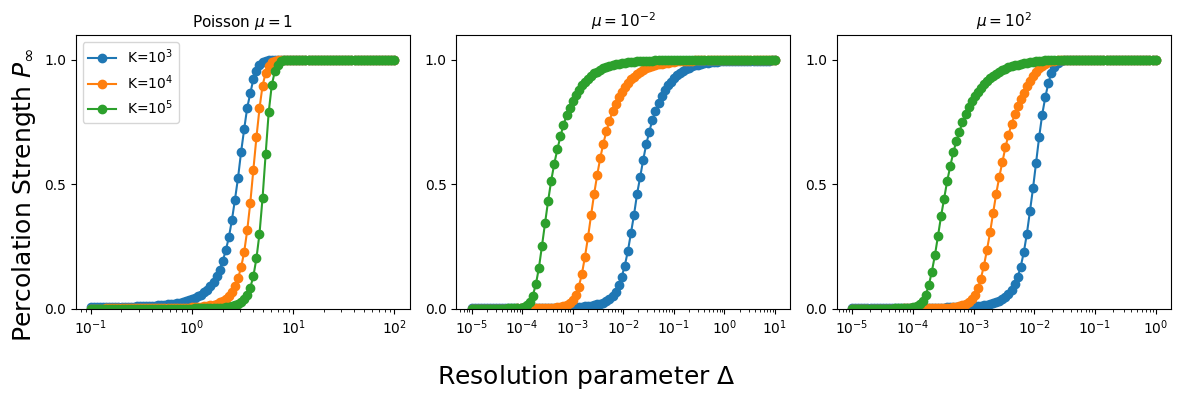
\includegraphics[width=0.8\textwidth]{phase bivariate stationary 10-2.png}
    \caption{Percolation phase diagrams averaged over $R=1000$ ``stationary'' signals of $K=10^5$ events. $\left( n_{EE}=n_{EI}=1.5, n_{IE}=-0.5 \right)$}
    \label{f:phase_diagram_coupled oscilatory}
\end{figure}

\begin{figure}[H]
    \centering
    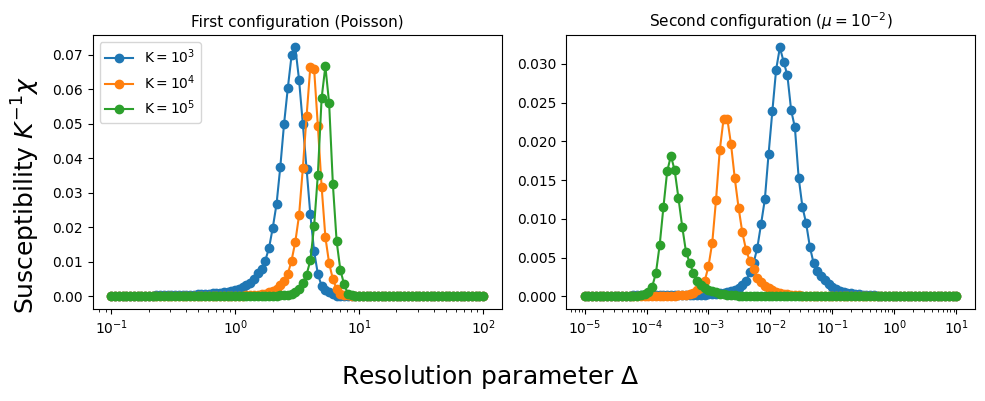
\includegraphics[width=0.8\textwidth]{susceptibilidad bivariate stationary 10-2.png}
    \caption{Susceptibility $\chi$ normalized to $K$ associated with the above phase diagram.}
    \label{f:susceptibilidad_coupled oscilatory}
\end{figure}

We note an almost identical behaviour to the one shown in the case of the ``pseudo-critical'' signals, with just a single transition around $\Delta^*\approx 2\cdot 10^{-4}$ for $10^5$ events, 
agreeing with the universality class of 1D percolation. In this case, as Figure \ref{f: stats oscilatory} 
indicates, the exponents are indeed $\alpha=\tau=2$ but exponentially decaying.

\begin{figure}[H]
    \centering
    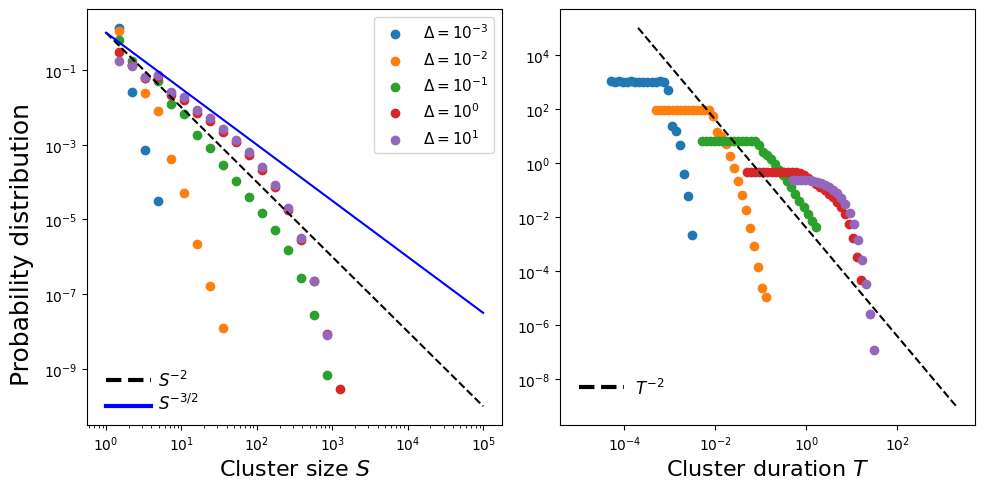
\includegraphics[width=0.8\textwidth]{stats stationary bivariate 10-2.png}
    \caption{Avalanche statistics of $K=10^5$ events for ``stationary'' signals of two coupled Hawkes processes. Histograms have been calculated over $R=1000$ time series.}
    \label{f: stats oscilatory}
\end{figure}

To conclude the chapter, in Table \ref{tab: all exponents} are presented all the exponents obtained for the different configurations studied.


\begin{table}[H]
    \centering
    \caption{Power-law exponents for every configuration studied.}
    \label{tab: all exponents}
    \begin{tabular}{@{}cccccccc@{}}
    \toprule
    \multicolumn{1}{c}{} & \multicolumn{1}{c}{Poisson} & \multicolumn{2}{c}{n=1}      & \multicolumn{2}{c}{n=2}      & \multicolumn{2}{c}{Bivariate with excitation and inhibiotn} \\ \midrule
                         & $\mu=1$                     & $\mu=10^{-4}$ & $\mu=10^{2}$ & $\mu=10^{-4}$ & $\mu=10^{2}$ & ``Pseudo-critical''  & ``Stationary'' \\
    \alpha & 2 & 2$\overset{\Delta\uparrow}{\longrightarrow} 3/2$ & 2 & 2 & 2 & 2$\overset{\Delta\uparrow}{\longrightarrow} 3/2$  & $\sim$ 2 (damped) \\
    \tau   & 2 & 2          & 2 & 2 & 2 & 2          & $\sim$ 2 (damped) \\ \bottomrule
    \end{tabular}
\end{table}